\section{Results}
For country-product bi-partite networks,  Caldarelli et al. \cite{caldarelli2012network} found that the ranking of countries correlates reasonably well with their ranking in terms of GDP, after calibration of $\alpha$ and $\beta$ (Pearson correlation $\approx 0.4$ for $\alpha \approx 1.1$ and $\beta \approx 0.8$). Similarly, we studied the correlations of the editors/articles ranking model with grand-truth exogenous values. We studied how these correlations evolve as more edits are contributed to a category of Wikipedia articles. Finally, we investigated the values of calibrated $\alpha$ and $\beta$ in the context of Wikipedia open collaboration.

Figure \ref{fig:rhotime} shows the evolution of the rank correlation (Spearman $\rho$) between $\mathbf{w}^*_e$ and $\mathbf{v}^*_e$, and $\mathbf{w}^*_a$ and $\mathbf{v}_a$ respectively, as a function of time for each of the ten categories ($\alpha$ and $\beta$ are calibrated for each category and each snapshot so that maximum correlation is found). The maximum rank correlation is obtained by numerical optimization {\bf [please describe shortly the method employed]}. The correlations are generally quite high ( $ 0.46 < \rho_e < 0.75$ with $\langle \rho_e\rangle = 0.64$ for editors and $0.57 < \rho_a < 0.91$ with $\langle \rho_a\rangle = 0.72$ ). Yet the rank correlations of editors remain overall smaller than rank correlations obtained for articles. This difference might be due to the roughness of the grand truth for editors $v_e$, expressed in labor-hours, compared to the quality of $v_a$, which is an aggregate measure of five precise quality metrics. Nevertheless, the correlation of editors' ranking with $v_e$ increases: $\rho_e$ exhibits a convex increase over time, suggesting that it takes time (i.e., lots of edits) to capture well the expertise of editors as well as for editors. 

%{\bf [is there a unique set of $\alpha$ and $\beta$ for $\mathbf{w}^*_a$ and $\mathbf{w}^*_e$ ? Or do you calibrate $\alpha$ and $\beta$ for  $\mathbf{w}^*_a$ and then  $\mathbf{w}^*_e$ ?]}

 \begin{figure}[!t]
 \centering
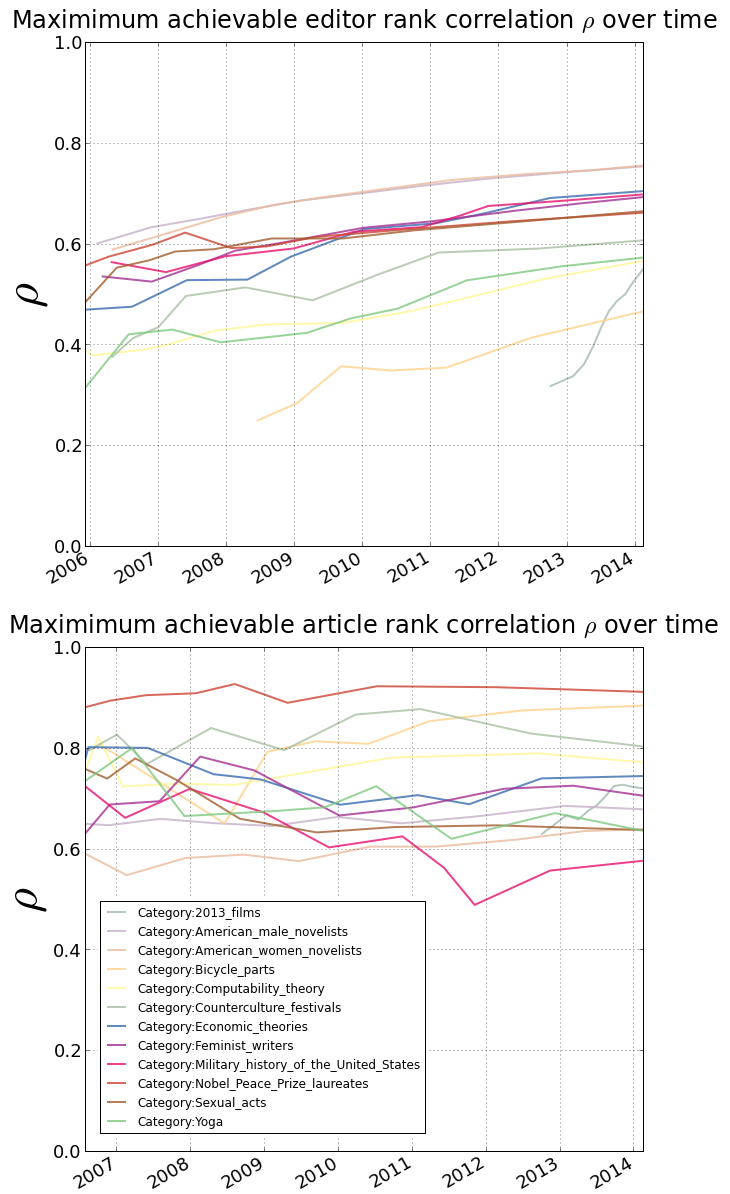
\includegraphics[width=0.9\columnwidth]{Figures/rho_combined.png}.
\caption{Evolution of Spearman $\rho$ rank correlations between the ranking obtained from the calibrated model and the grand-truth values for each category and for editors (upper panel)  and articles (lower panel). The correlations are generally quite high : $ 0.46 < \rho_e < 0.75$ with $\langle \rho_e\rangle = 0.64$ for editors and $0.57 < \rho_a < 0.91$ with $\langle \rho_a\rangle = 0.72$. $\rho_{a}$  is stable over time, which means that the quality of articles can be pretty well captured early on by the model. However, $\rho_e$ exhibits a convex increase over time, suggesting that it takes time (i.e., lots of edits) to capture well the expertise of editors.{\it [please add a label for the x-axis (i.e., Time [years]) and change $\rho$ into $\rho_e$ and $\rho_a$ respectively. You can remove the titles above the  plots]}}
 \label{fig:rhotime}
 \end{figure}

We now turn to the values of $\alpha$ and $\beta$ for which best correlation is achieved.  Figure \ref{fig:landscape} shows typical landscapes of correlation as a function of $\alpha$ and $\beta$ for editors and articles. It appears that there is no single value of $\alpha$ and $\beta$ for best correlation, but rather some areas (showed by the contour line on Figure \ref{fig:landscape} as the 90th percentile of the rank correlation). The contour line exhibits a linear function between $\alpha$ and $\beta$. For articles, the relationship is typically of the type $\alpha = - b \beta + 1$ for $\beta >0$ with $b$ varying for each category. {\bf [it would make sense to actually evaluate $b$, for instance by making regression of all points above the 90th percentile]} For editors, the relationship is $\alpha = 0$ for $\beta < ??$ {\bf [complete the value once the related plot has been added]}. 

\begin{figure}[!t]
\centering
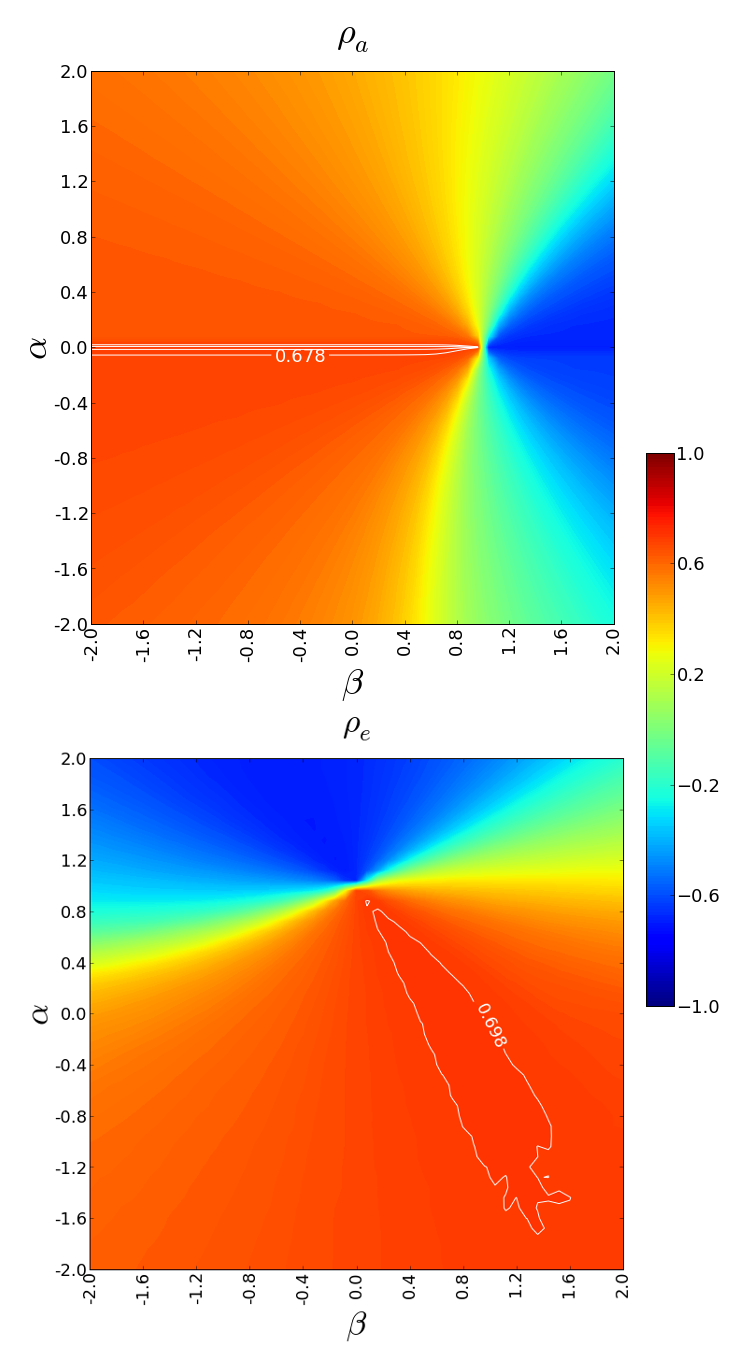
\includegraphics[width=0.9\columnwidth]{Figures/contour_fem_combined.png}.
\caption{Typical landscape of maximum correlation as a function of $\alpha$ and $\beta$ for editors (upper panel) and articles (lower panel). The contour line shows the 90th percentile of the rank correlation over the landscape. It typically displays a linear function between $\alpha$ and $\beta$. For articles, the relationship is typically of the type $\alpha = - b \beta + 1$ for $\beta >0$ or $\alpha = b \beta + 1$ for $\beta < 0$ with $b>0$ varying for each category. For editors, the relationship is $\alpha = 0$ for $\beta < ??$. {\it please add the corresponding figure for editors.  that would be great if you could make the labels ($\alpha$ and $\beta$) WAY bigger. You can also get remove the title. The cherry on the cake would be to have the color bar equal or smaller than the vertical dimension of the landscape, with keeping the landscape as a square rather than a rectangle.}}
\label{fig:landscape}
\end{figure}


{\bf [it would be great to have a table that shows the values of $\alpha$ and $\beta$ for articles and editors and for each category (last snapshot). By the way, my latest impression from the contour line plots is that a optimal point can be found]}


%\clearpage


%\subsection{Article-Editor Ranking Calibration}
%
%Having our endogenous and exogenous variables now, we perform tests to
%$\underset{\alpha, \beta}{\operatorname{argmax}} \rho(\alpha, \beta)$, the pair that maximizes our spearman rank correlation between  $\mathbf{w^{*}_{e}}$ and $v_e$. We also do so for $\mathbf{w^{*}_{a}}$ and $v_a$.
%
%First we used a general purpose maximizing algorithm to find maximizing values. Secondly we performed a grid search with visual inspection. Overall we find smooth landscapes. The two methods verified each other's results. \ref{fig:contour_fem} shows the correlation landscape for Category:Feminist Writers calibrating both articles and editors.
%
%The results of calibrating our model are encouraging as we find high correlations between the results of our $w^*_e$ algorithm and our exogenous variables $v$. 
%
%We define $\rho$ at the maximum achievable spearman rank correlation between $w^*$ and $v$ for editors or articles, by category, and over time. The variation of $\rho$, by for editor for any category ranges from 0.75 to 0.46 with a mean 0.64.  That same statistic for articles is articles from 0.91 to 0.57 with a mean of 0.72, which is overall higher.
%
% 
%From snapshotting we see view $\rho$ as  a function of time. In the case of editors we see increasing trends in all categories over time in an asymptotic way. This means that $w^*_e$ benefits from incorporating more contribution history. That is, as a category matures we can better predict successful editors from which articles they edit. As for being able to predict article quality, from the start of a category's history the correlations remain high and  stable. It is easier to predict an articles quality based on who has edited it.  \ref{fig:rhotime}
%
%\begin{figure}[!t]
%\centering
%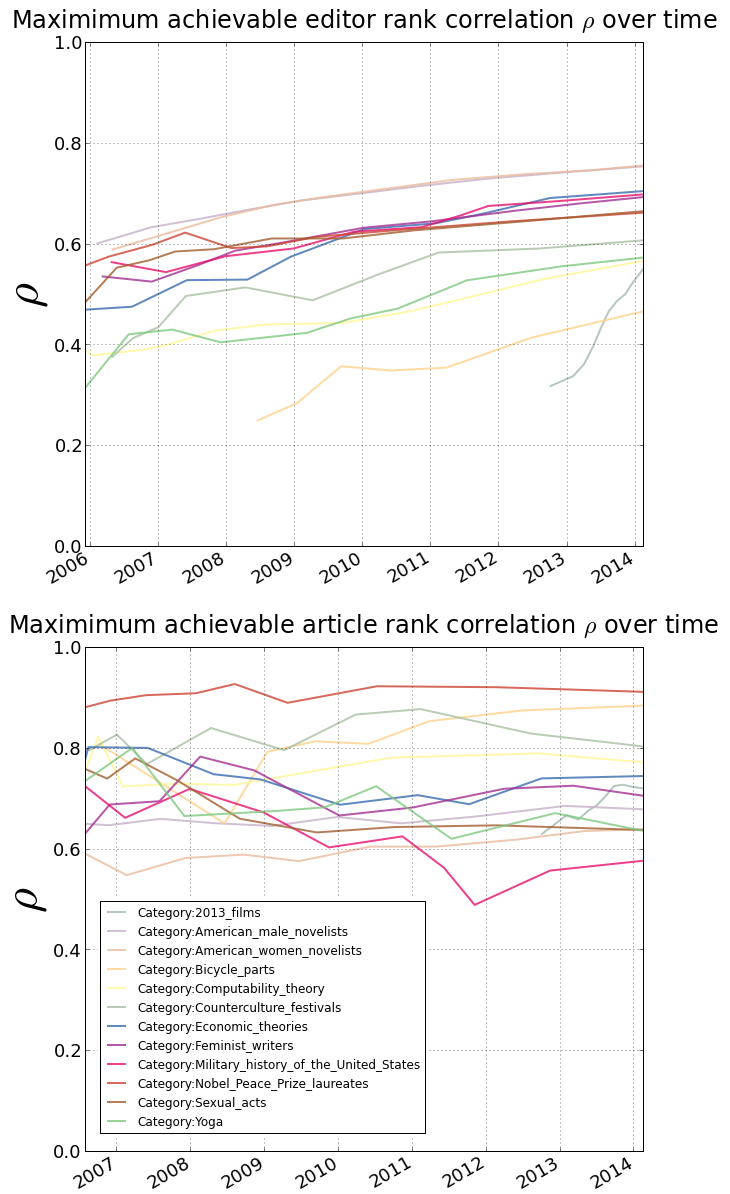
\includegraphics[width=0.9\columnwidth]{Figures/rho_combined.png}.
%\caption{$\rho$ over time, by category and type}
%\label{fig:rhotime}
%\end{figure}
%
%
%\subsection{Negative values of $\alpha$ and $\beta$}
%Another surprising result is that we find at times, negative values for $\alpha$ and $\beta$.
%
%To understand the results, we must have a firm grasp on what $\alpha$ and $\beta$ mean. They are more easily understood by roughly rewriting $\mathbf{w^*}$ as:
%\begin{equation}
%\begin{cases}
%w^{*}_{e} \sim k^{1-\beta}_{e} \langle k_{a}^{-\alpha}\rangle_e \\
%w^{*}_{a} \sim k^{1-\alpha}_{a} \langle k_{e}^{-\beta}\rangle_a
%\end{cases} \label{eqsim}
%\end{equation}
%
%Our solution spaces are not single point but a 2-dimensional area, similar to what found in \cite{caldarelli2012network}. A reason for this is the fact that we are using the spearman ranking correlation, once a ranking is achieved, $\alpha$ and $\beta$ can perturb without adjusting the ranking. 
%
%In these areas we see trends in there being important axes shown by the maximizing segments, which represent a several explanations for the article behaviour behaviour.
%
%With regards to \eqref{eqsim}, we can see the similarity of $w^*$ is related to the product of two expression. Values of $\alpha$ and $\beta$ can make the one of the product approach one or and so the other parameter may dominate. In the article plot of \ref{fig:contour_fem} our solution spaces moves linearly from $0 <\alpha <1 , \beta \approx 0$ meaning that successful editors are charcterized, by an equal balance of their edit count, and the average article quality of articles they've edited. At the other end $\alpha < - 1 , \beta > 1$ anti-importance of their how man articles they've edited, but high importance on the quality of edits.
%
%This seems quite natural to say, but $\alpha$ and $\beta$ need not vary together at all, and could be in different quadrants of the landscape each describing a different success strategy.
%
%\begin{figure}[!t]
%\centering
%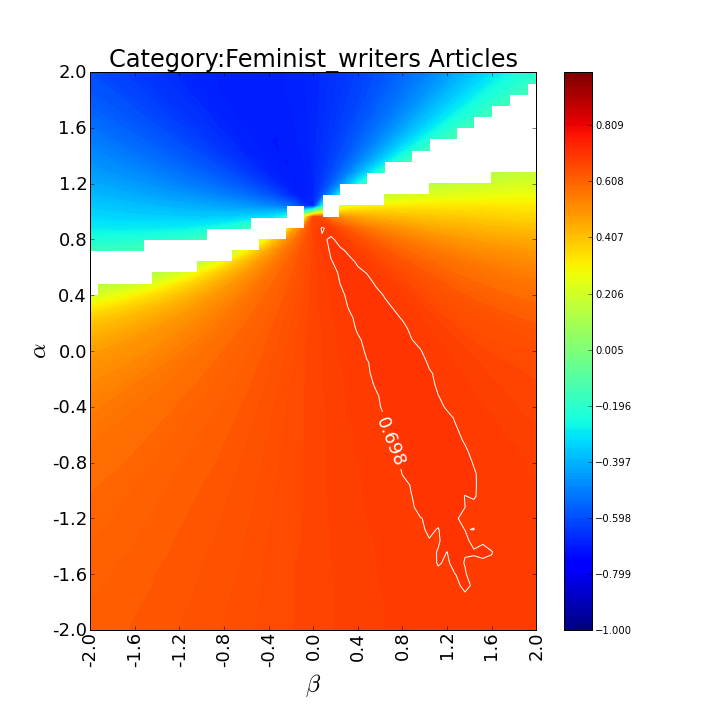
\includegraphics[width=0.9\columnwidth]{Figures/contour_fem.png}.
%\caption{Heatmaps of Spearman Rank Correlation between endogenous and exogenous ranks, 95$^{th}$ percentile  of correlations circled
%Upper panel: articles - $w^*_a ~ v_a$
%Lower panel editors - $w^*_e ~ v_e$
%White indicates that correlation was not significant $p<0.05$ } 
%\label{fig:contour_fem}
%\end{figure}
%
%\subsection{$\rho$ increases over time.}

	



